% !Mode:: "TeX:UTF-8"
\documentclass[QAofGroup.tex]{subfiles}

\begin{document}
%-=-=-=-=-=-=-=-=-=-=-=-=-=-=-=-=-=-=-=-=-=-=-=-=
%
%	CHAPTER
%
%-=-=-=-=-=-=-=-=-=-=-=-=-=-=-=-=-=-=-=-=-=-=-=-=

%%================================================================
\chapter{20171028}\label{ch1028}

%----------------------------------------------------------------------------------------
\begin{qst}\label{Q2017102801}
请问我刚安装的TL2017+texstudio,编译预览,为什么无法用ctrl+单击跳转到代码处?
电脑默认的pdf阅读器是adobe acrobat DC,谢谢!
现在加了一个sumartpdf。\index{SumartPDF}

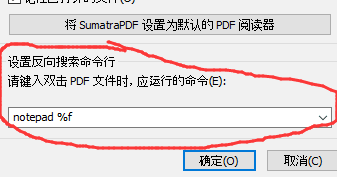
\includegraphics[width=0.85\textwidth]{pic01.png}

这里要添加什么命令才可以呢?
\end{qst}
\ans \verb|"D:\Programfiles\texstudio-2.12.4\texstudio.exe" "%f" -line %l|

\begin{qst}\label{Q2017102802}
用TeX写实验报告为什么section上下的空间很大?
\end{qst}
\ans 你去看看section的定义就知道了, 间距都可以重新设置。

\begin{qst}\label{Q2017102803}
此数学符号$\displaystyle\lim\limits_{n\to\infty\atop m\to\infty}$怎么敲打?
\end{qst}
\ans \verb|\lim\limits_{n\to\infty\atop m\to\infty}|\index{atop}

\begin{qst}\label{Q2017102804}
我试着用figure和caption环境,结果表格这些总是跑掉,怎么办?
\end{qst}
\ans “总是跑掉”用了\verb|\begin{figure}[hbt!]| 吗?那个感叹号不能少。
\end{document} 